\documentclass[fontsize=12]{article}

\usepackage{spotted}
\title{Hand Luggage Scanning}
\author{Week 10, Spotted in the Wild}
\date{Tom Cassar}

\begin{document}

\maketitle

This Easter, I flew to South Africa to visit my friend from university. The
journey there meant going through airport security. At Gatwick, my hand luggage
was flagged for a manual search which means I got to see the image of the
luggage scan. This reminded me of the Week 10 content on fMRI imaging.

\begin{figure}[H]
    \centering
    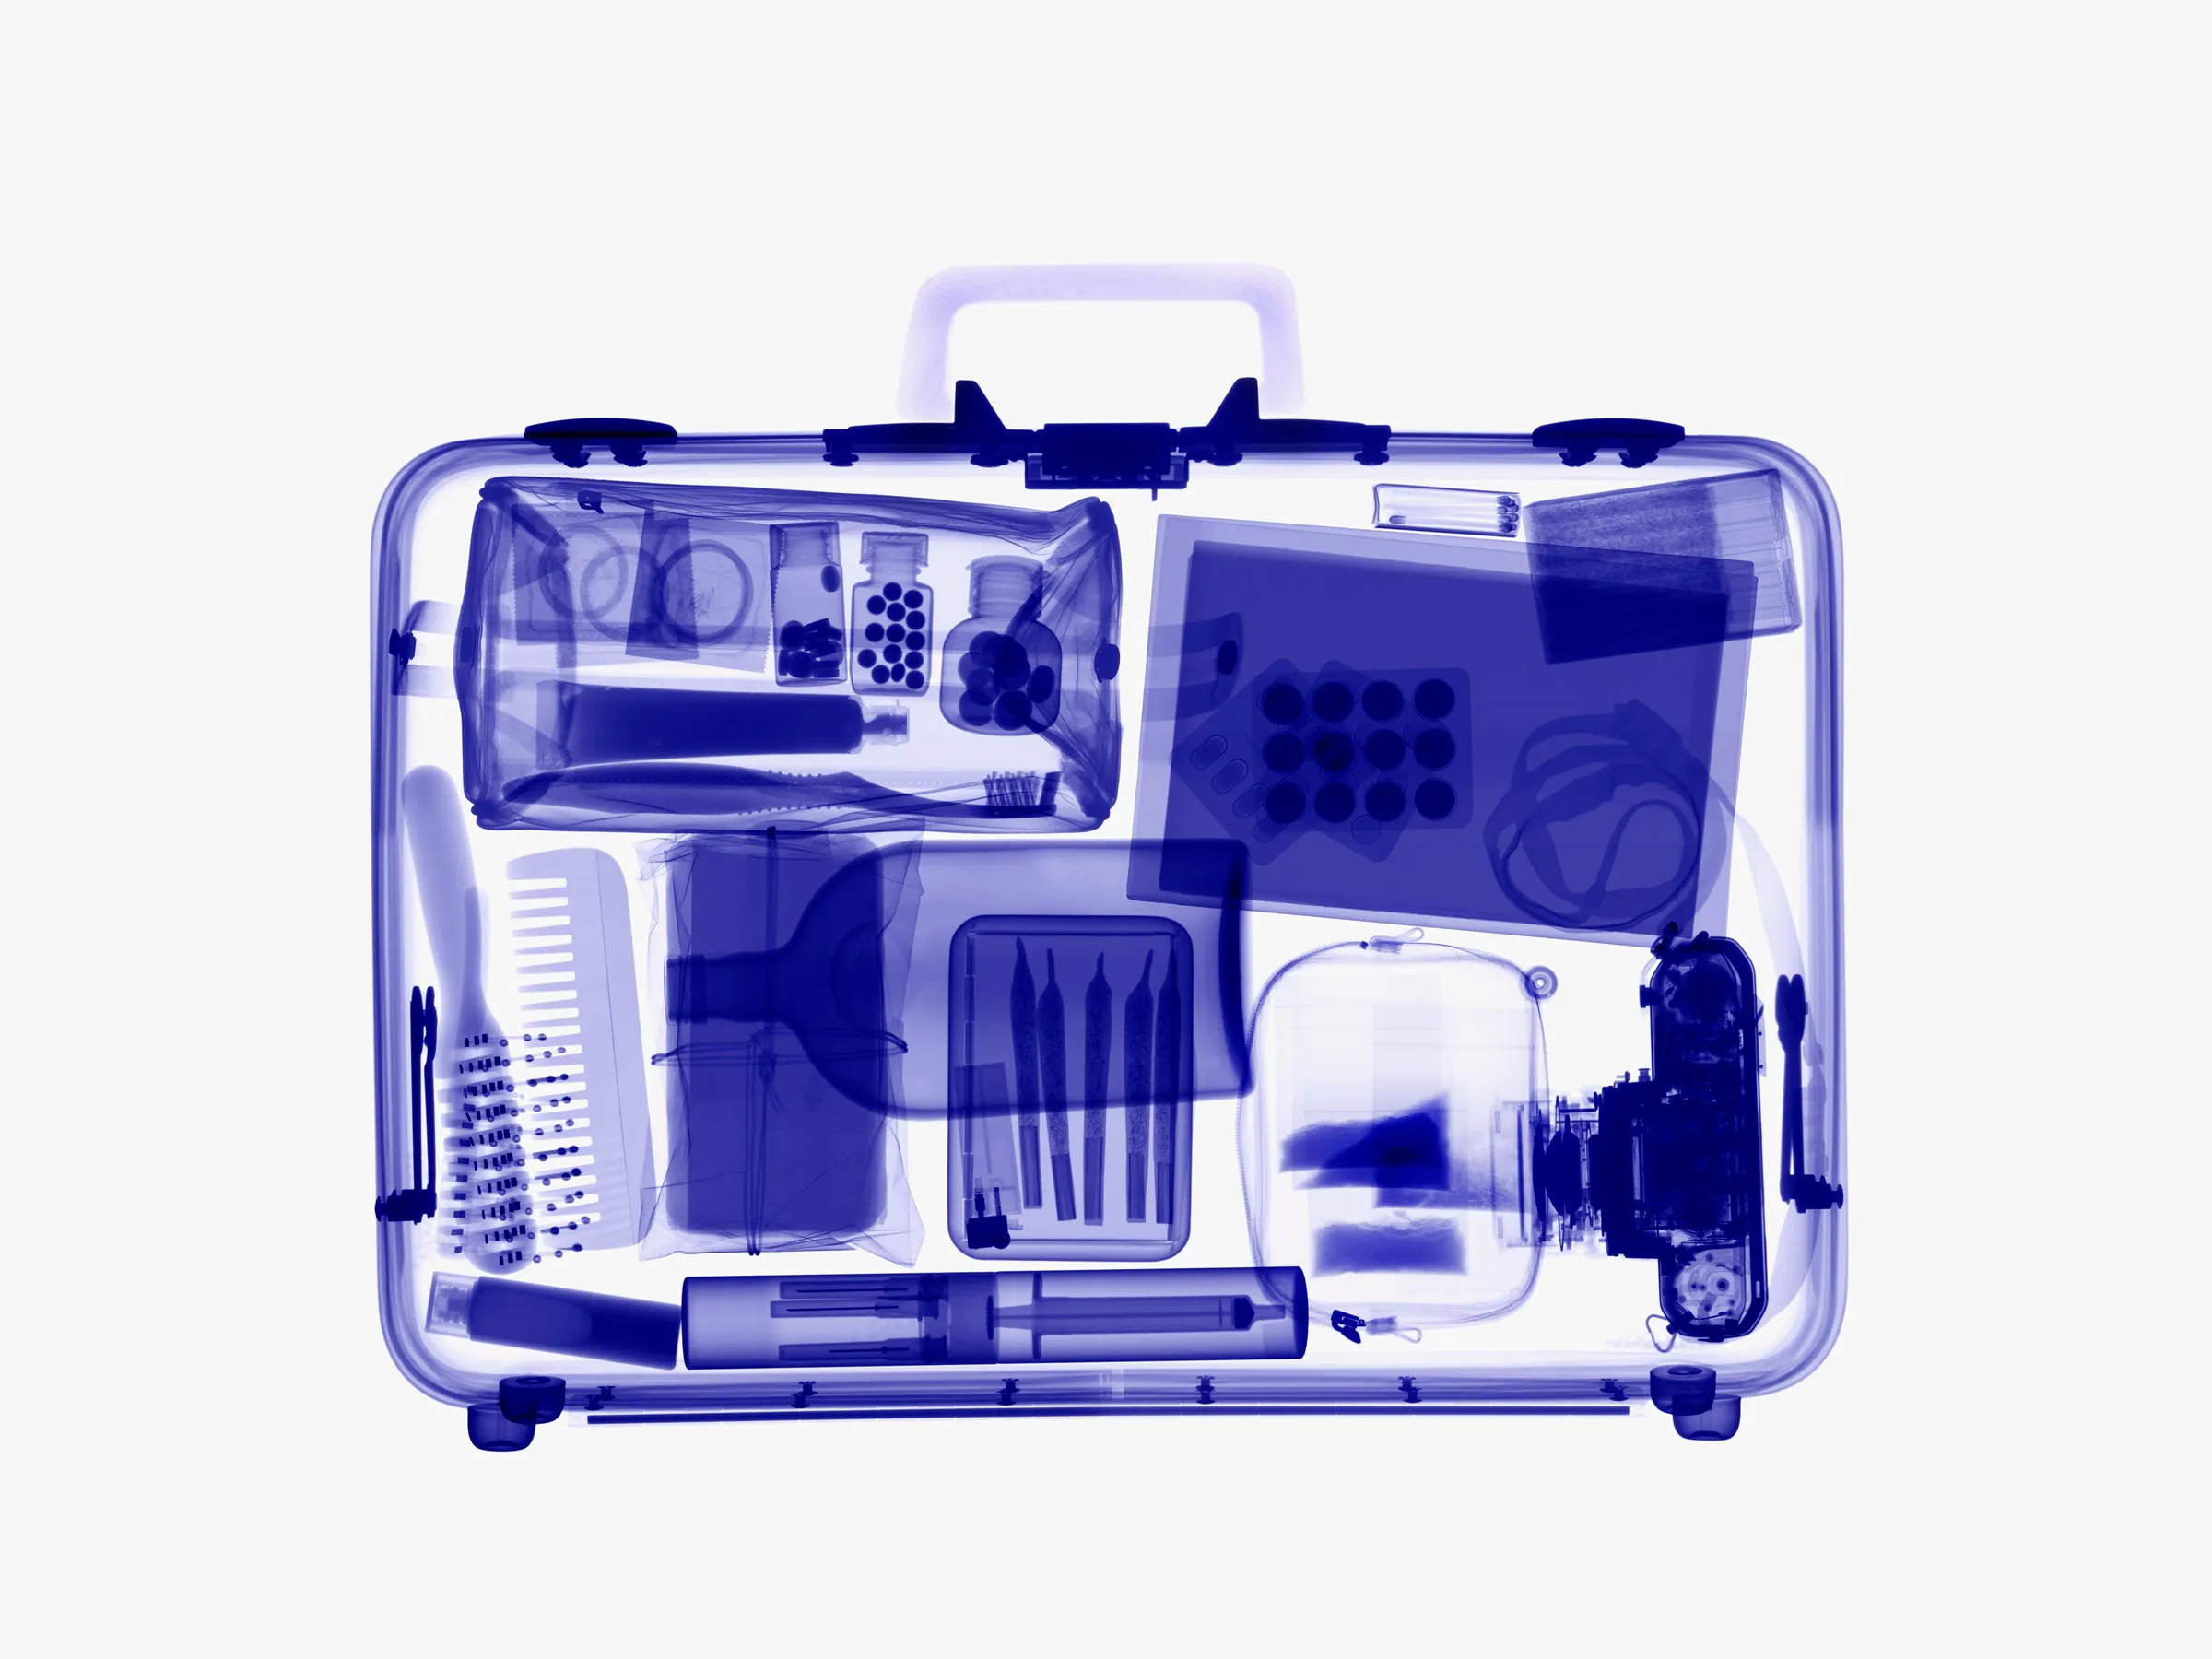
\includegraphics[width=0.6 \linewidth]{./img/suitcasescan-TA.png} 
    \caption{An example of a hand luggage being scanned (I wasn't allowed to
    take a photo of my own luggage scan)}\label{fig:illusion}
\end{figure}

Both processes are a non-invasive imaging technique which are used to ``look
inside'' objects for classification. fMRI classifies active brain regions and
the luggage scanners classify safe/suspicious luggage.

fMRI scans are often used medically in diagnostics to identify abnormalities in
brain areas of interest. Exploratory studies are also often conducted with fMRI.

Baggage scans don't use the MRI technology but something different entirely.
There are similarities in the post-processing of each technology though. fMRI
colours by density, whereas baggage scans are radiation based.

\end{document}



